\documentclass{oblivoir}
\usepackage{amsmath,amssymb,amsthm,kotex,mdframed,paralist,kswrapfig}

\newcounter{num}
\newcommand{\prob}
{\bigskip\noindent\refstepcounter{num}\textbf{문제 \arabic{num})}\par}

\newcommand{\ans}{{\raggedleft\textbf{답 : (\qquad\qquad\qquad\qquad\qquad\qquad)}
\par}\bigskip\bigskip}


%%%
\begin{document}
\Large

\title{승재 12 - 6학년 2학기 - 05}
\author{}
\date{\today}
\maketitle
%\tableofcontents

\newpage

%
\prob
민희와 효연이는 사과 두 개를 먹었습니다.
민희와 효연이가 먹은 사과의 양을 가장 간단한 자연수의 비로 나타내세요.

\ans

\begin{figure}[h!]
\centering
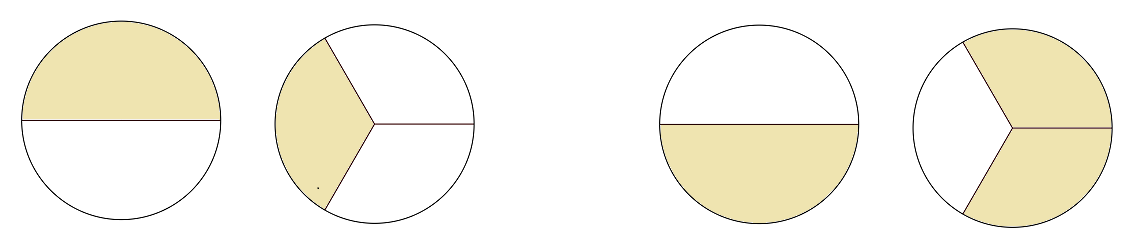
\includegraphics[width=0.9\textwidth]{01}

민희가 먹은 사과\qquad\qquad\qquad\qquad\quad 효연이가 먹은 사과
\end{figure}


%
\prob
지호와 영신이는 사과 두 개를 먹었습니다.
지호와 영신이가 먹은 사과의 양을 가장 간단한 자연수의 비로 나타내세요.

\ans

\begin{figure}[h!]
\centering
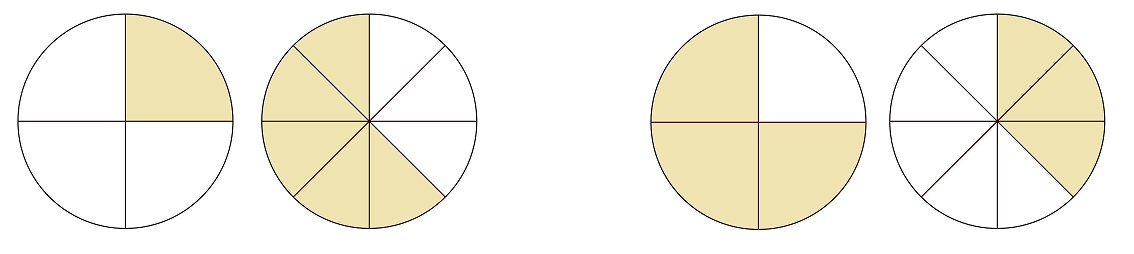
\includegraphics[width=0.9\textwidth]{02}

지호가 먹은 사과\qquad\qquad\qquad\qquad\quad 영신이가 먹은 사과
\end{figure}
\newpage

%
\prob
지수와 효정이는 사과 두 개를 먹었습니다.
지수와 효정이가 먹은 사과의 양을 가장 간단한 자연수의 비로 나타내세요.

\ans

\begin{figure}[h!]
\centering
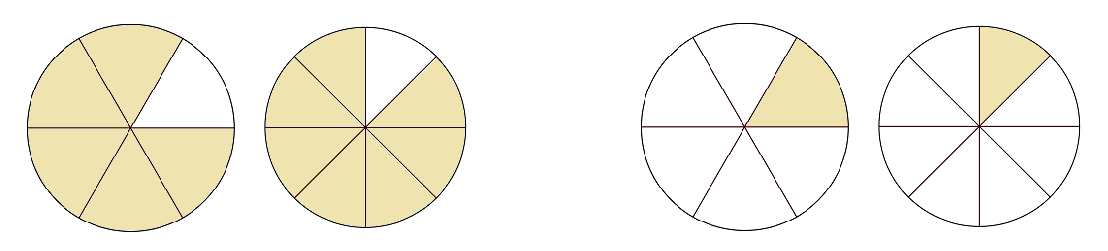
\includegraphics[width=0.9\textwidth]{03}

지수가 먹은 사과\qquad\qquad\qquad\qquad\quad 효정이가 먹은 사과
\end{figure}

%
\prob
윤지와 준호는 사과 세 개를 먹었습니다.
윤지와 준호가 먹은 사과의 양을 가장 간단한 자연수의 비로 나타내세요.

\ans

\begin{figure}[h!]
\centering
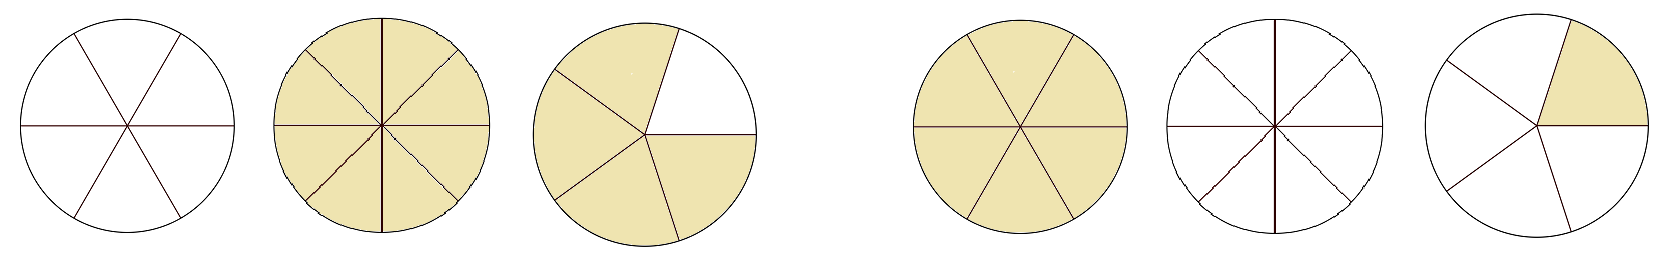
\includegraphics[width=0.9\textwidth]{04}

윤지가 먹은 사과\qquad\qquad\qquad\qquad\quad 준호가 먹은 사과
\end{figure}

\newpage

%
\prob
다음은 한 변의 길이가 1cm인 쌓기나무를 사용하여 수를 나타낸 것입니다.

\begin{figure}[h!]
\centering
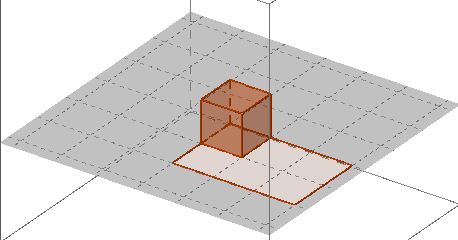
\includegraphics[width=0.45\textwidth]{05-001}
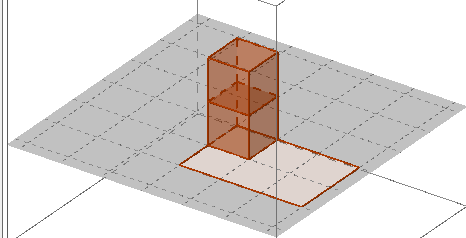
\includegraphics[width=0.45\textwidth]{05-002}

1\qquad\qquad\qquad\qquad\qquad\qquad\qquad\qquad2
\bigskip

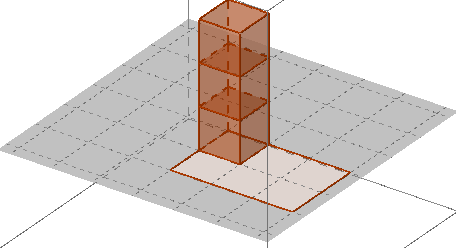
\includegraphics[width=0.45\textwidth]{05-003}
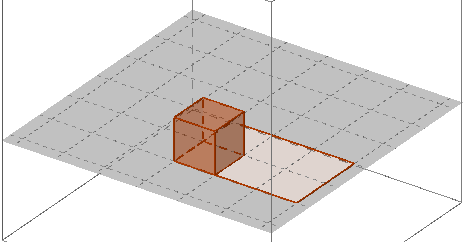
\includegraphics[width=0.45\textwidth]{05-004}

3\qquad\qquad\qquad\qquad\qquad\qquad\qquad\qquad4
\bigskip

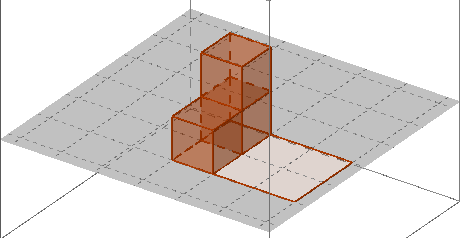
\includegraphics[width=0.45\textwidth]{05-006}
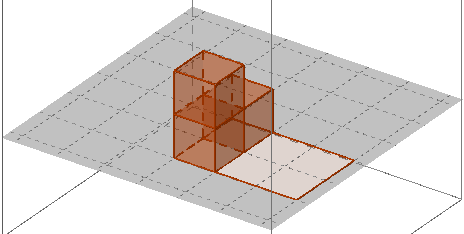
\includegraphics[width=0.45\textwidth]{05-009}

6\qquad\qquad\qquad\qquad\qquad\qquad\qquad\qquad9
\bigskip

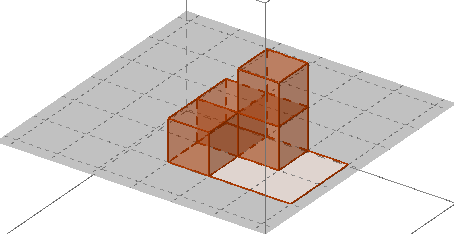
\includegraphics[width=0.45\textwidth]{05-025}
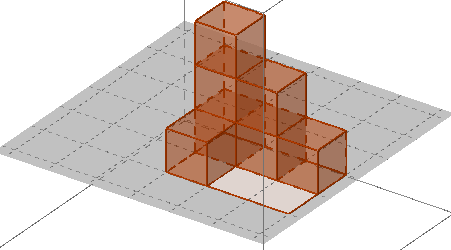
\includegraphics[width=0.45\textwidth]{05-127}

25\qquad\qquad\qquad\qquad\qquad\qquad\qquad\qquad127
\end{figure}
\newpage

(1) 도형들이 나타내는 수의 덧셈을 계산하여 도형으로 표현하세요.

\begin{figure}[h!]
\centering
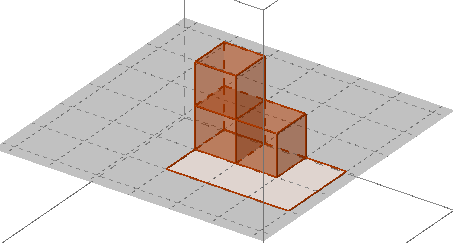
\includegraphics[width=0.45\textwidth]{05-012}
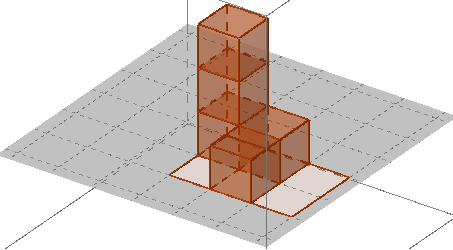
\includegraphics[width=0.45\textwidth]{05-053}

(\qquad\qquad\qquad)\qquad\qquad+\qquad\qquad(\qquad\qquad\qquad)\\

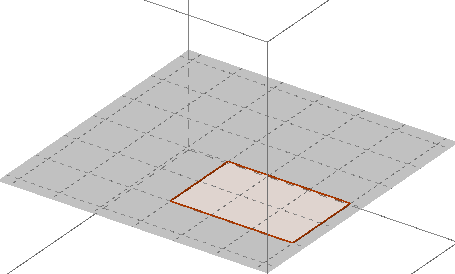
\includegraphics[width=0.45\textwidth]{05-000}

= (\qquad\qquad\qquad\qquad)
\bigskip\bigskip
%
%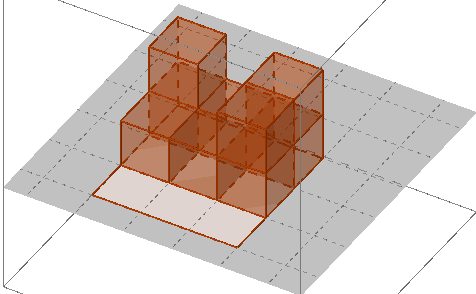
\includegraphics[width=0.45\textwidth]{05-845}
%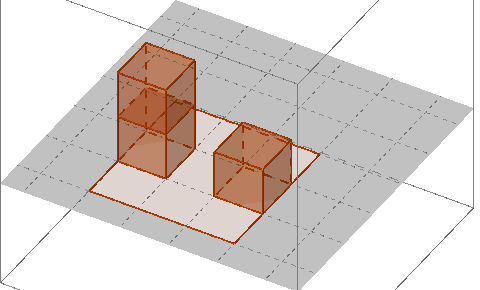
\includegraphics[width=0.45\textwidth]{05-306}
%
%(\qquad\qquad\qquad)\qquad\qquad\qquad\qquad\qquad(\qquad\qquad\qquad)
\end{figure}

(2) 45가 나타내는 도형에는 쌓기나무가 몇 개 사용됩니까?

\ans

(3) 263이 나타내는 도형에는 쌓기나무가 몇 개 사용됩니까?

\ans

(4) 17이 나타내는 도형의 겉넓이를 구하세요.

\ans

(5) 709가 나타내는 도형의 겉넓이를 구하세요.

\ans

\newpage


%
\prob
민희와 효연이는 바나나를 먹었습니다.
민희는 큰 바나나 1개를 먹었고 효연이는 큰 바나나 1개, 작은 바나나 4개를 먹었습니다.
민희와 효연이가 먹은 바나나의 양을 가장 간단한 자연수의 비로 나타내세요.
(단, 큰 바나나의 크기는 작은 바나나의 크기의 두 배입니다.)

\begin{figure}[h!]
\centering
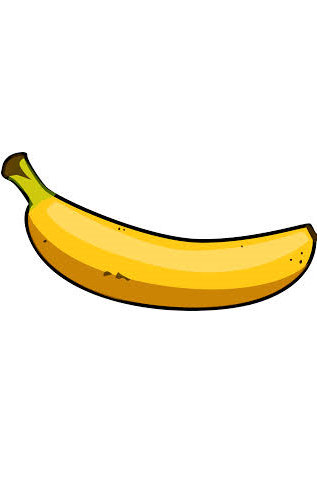
\includegraphics[width=0.4\textwidth]{06-1}
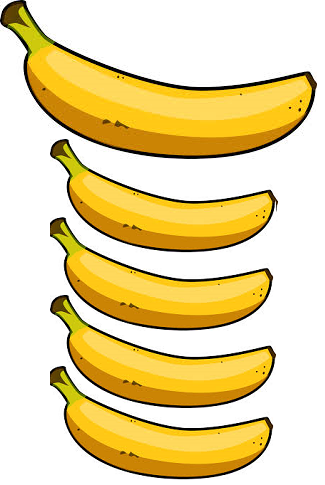
\includegraphics[width=0.4\textwidth]{06-2}

민희가 먹은 바나나 \qquad\qquad\quad 효연이가 먹은 바나나
\end{figure}

\ans

\newpage

%
\prob
지호와 영신이는 바나나를 먹었습니다.
지호는 큰 바나나 3개, 작은 바나나 3개를 먹었고
영신이는 큰 바나나 1개, 작은 바나나 5개를 먹었습니다.
지호와 영신이가 먹은 바나나의 양을 가장 간단한 자연수의 비로 나타내세요.
(단, 큰 바나나의 크기는 작은 바나나의 크기의 두 배입니다.)

\begin{figure}[h!]
\centering
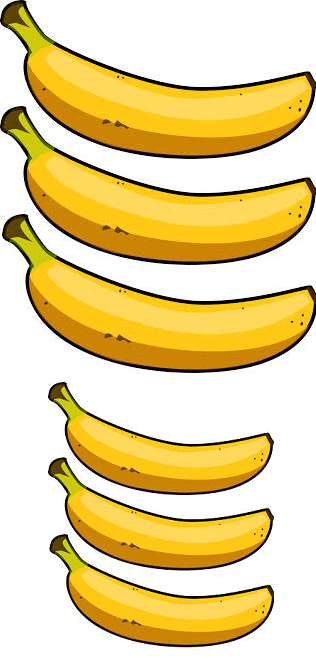
\includegraphics[width=0.4\textwidth]{07-1}
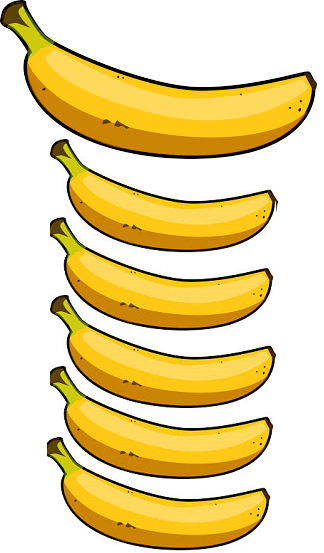
\includegraphics[width=0.4\textwidth]{07-2}

\qquad지호가 먹은 바나나\qquad\qquad\quad 영신이가 먹은 바나나
\end{figure}

\ans

\newpage

\prob
도형 (가)는 원의 1/4에 꼭 맞게 들어가는 정사각형을 나타낸 것이고
도형 (나)는 원의 1/4에 꼭 맞게 들어가는 삼각형을 나타낸 것입니다.


\begin{figure}[h!]
\centering
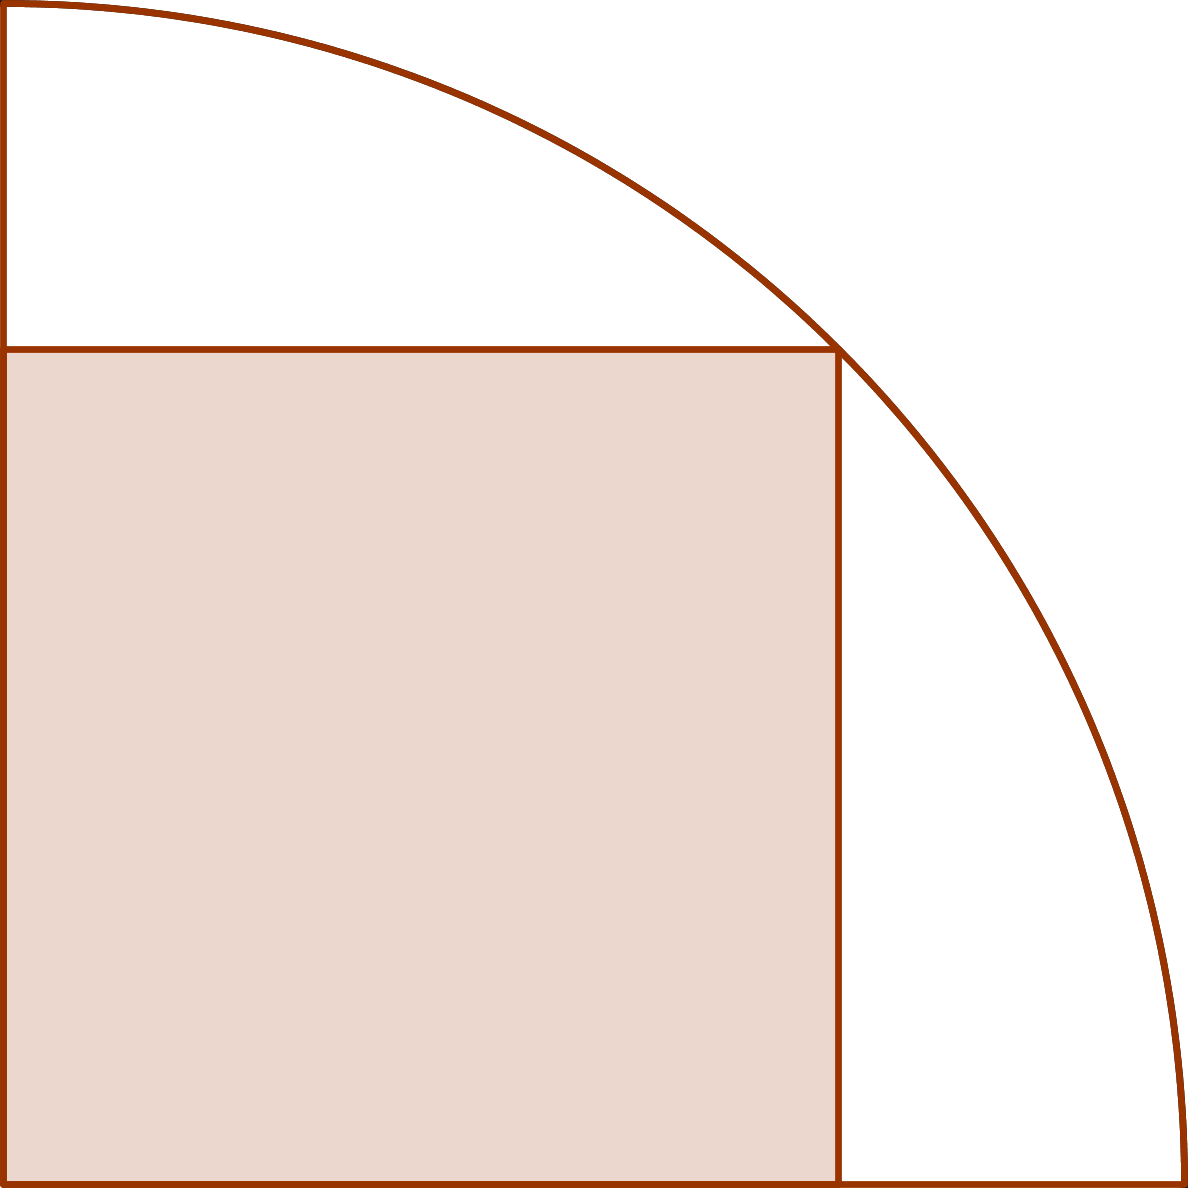
\includegraphics[width=0.25\textwidth]{08-1}
\qquad\qquad\qquad\qquad
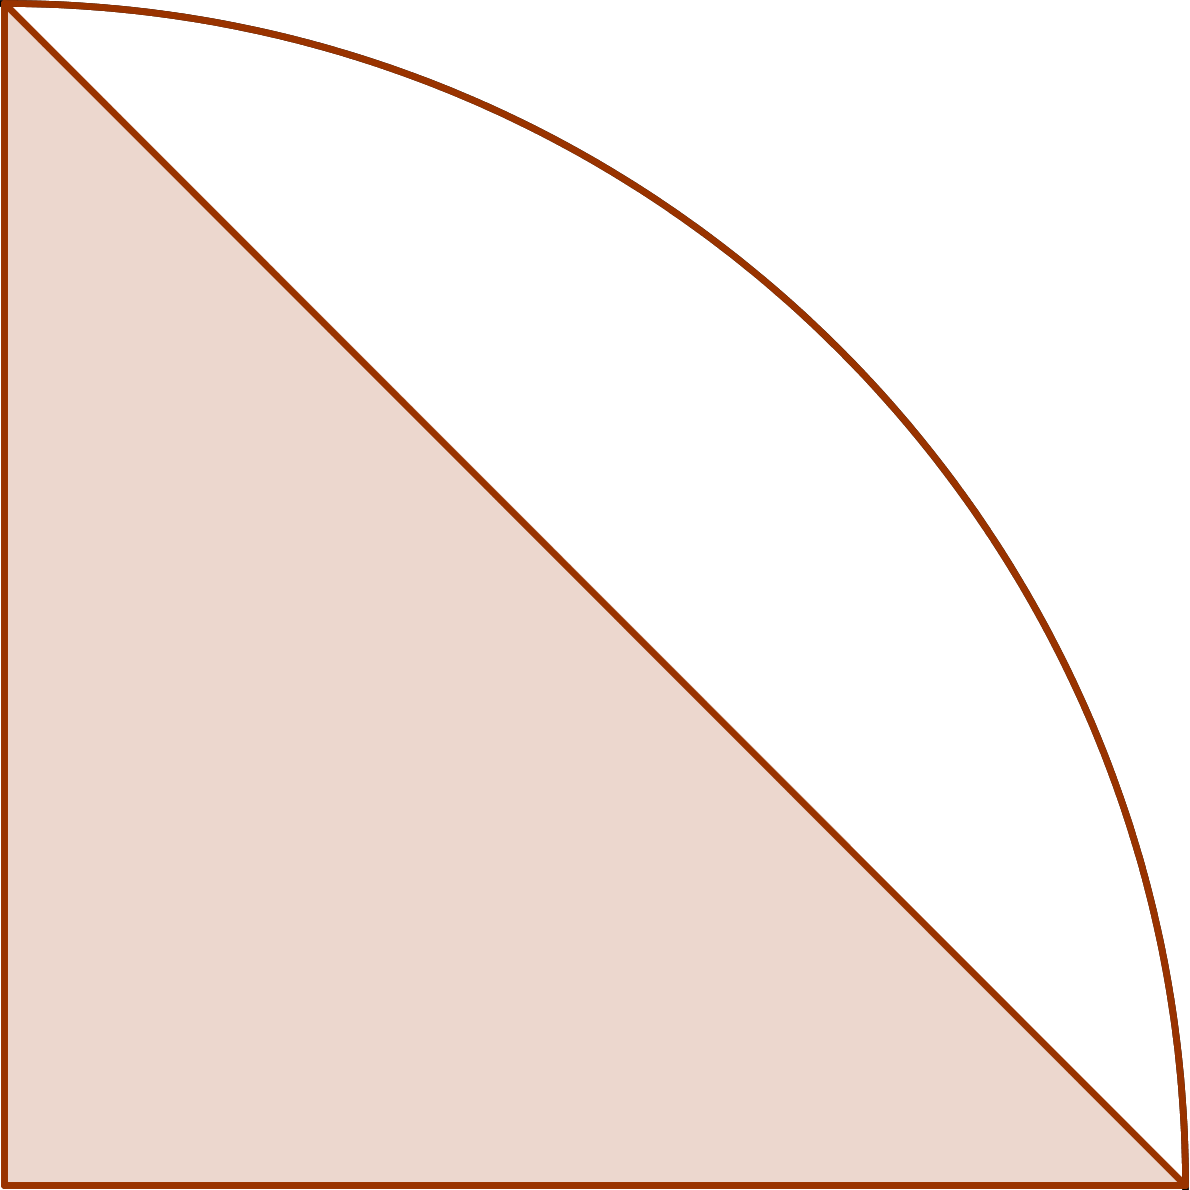
\includegraphics[width=0.25\textwidth]{08-2}

(가)\qquad\qquad\qquad\qquad\qquad\qquad\qquad\quad(나)
\end{figure}

두 원의 반지름이 10cm로 같을 때 (가)와 (나) 중 더 넓은 것은 무엇입니까?
\bigskip\bigskip

\textbf{답 : }

1. 도형 (가)가 도형 (나)보다 (\qquad)cm\(^2\)만큼 더 넓습니다.

2. 도형 (나)가 도형 (가)보다 (\qquad)cm\(^2\)만큼 더 넓습니다.

3. 도형 (가)와 도형 (나)는 넓이가 서로 같습니다.

\bigskip\bigskip
\textbf{힌트 : }
아래의 왼쪽 원에는 도형 (가)를 4개 채워 넣고 오른쪽 원에는 도형 (나)를 4개 채워 넣으세요.
그리고 만들어진 두 그림을 비교하세요.

\begin{figure}[h!]
\centering
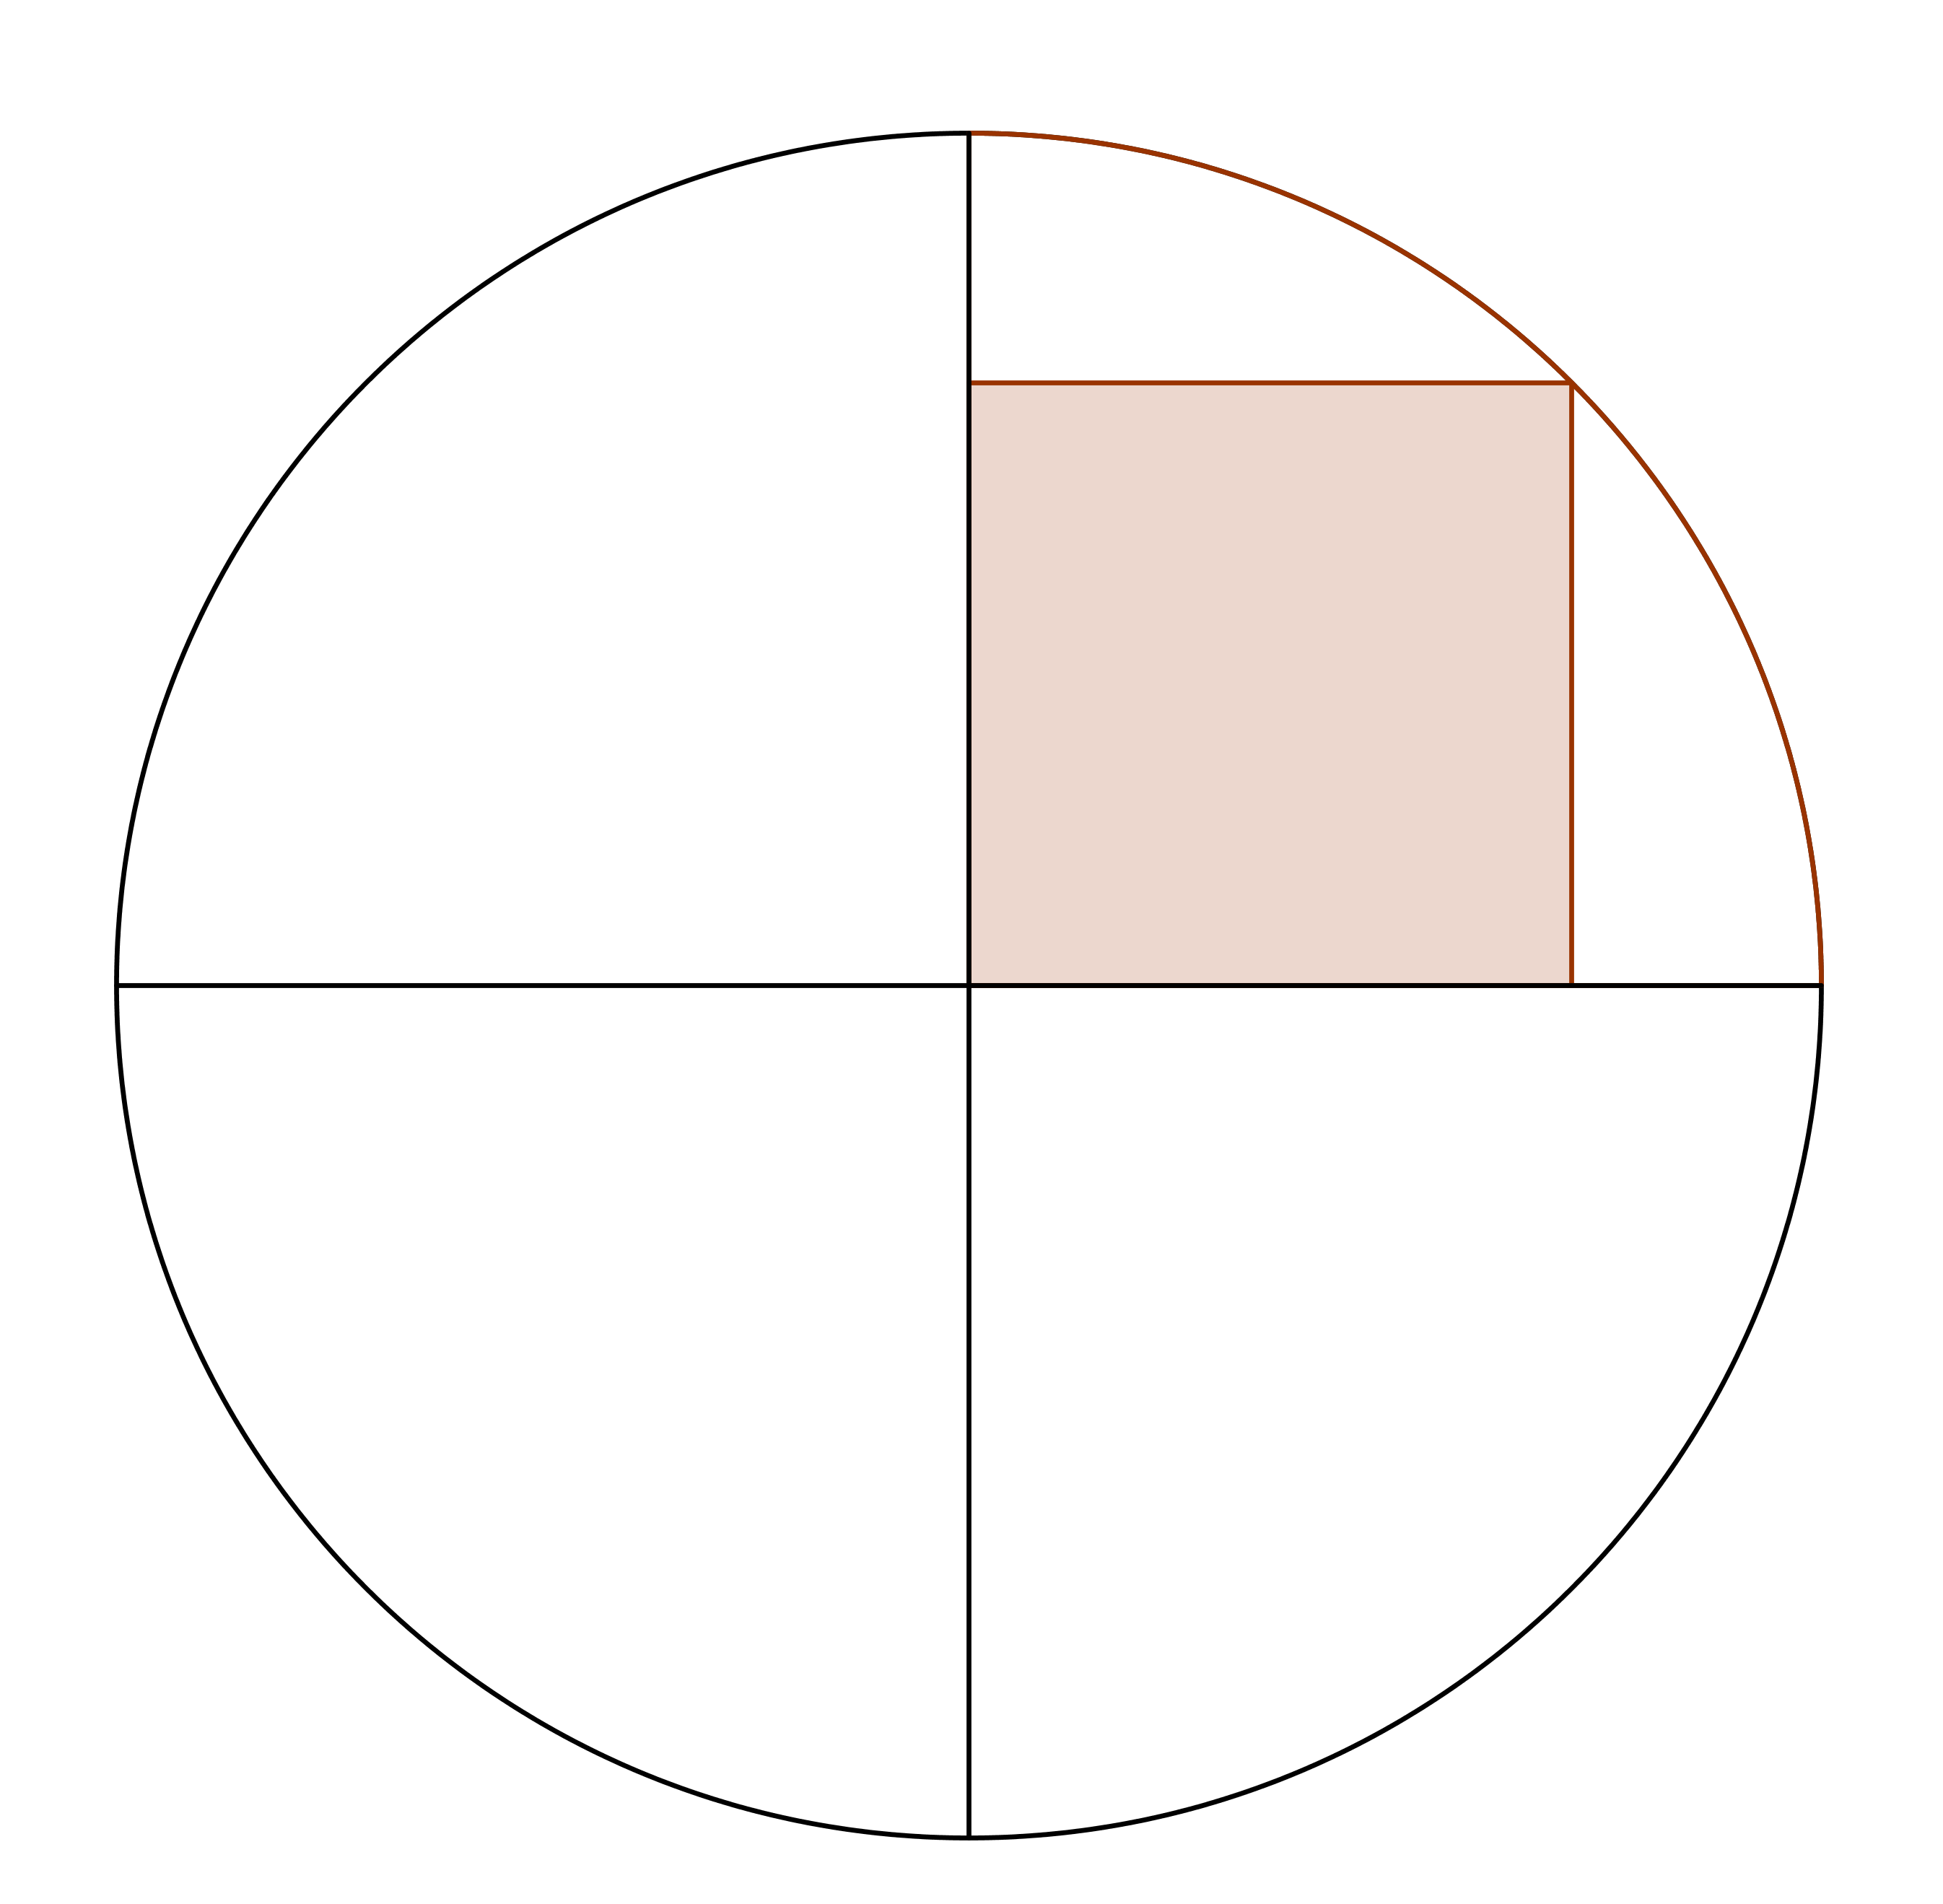
\includegraphics[width=0.3\textwidth]{08-3}
\qquad\qquad\qquad\qquad
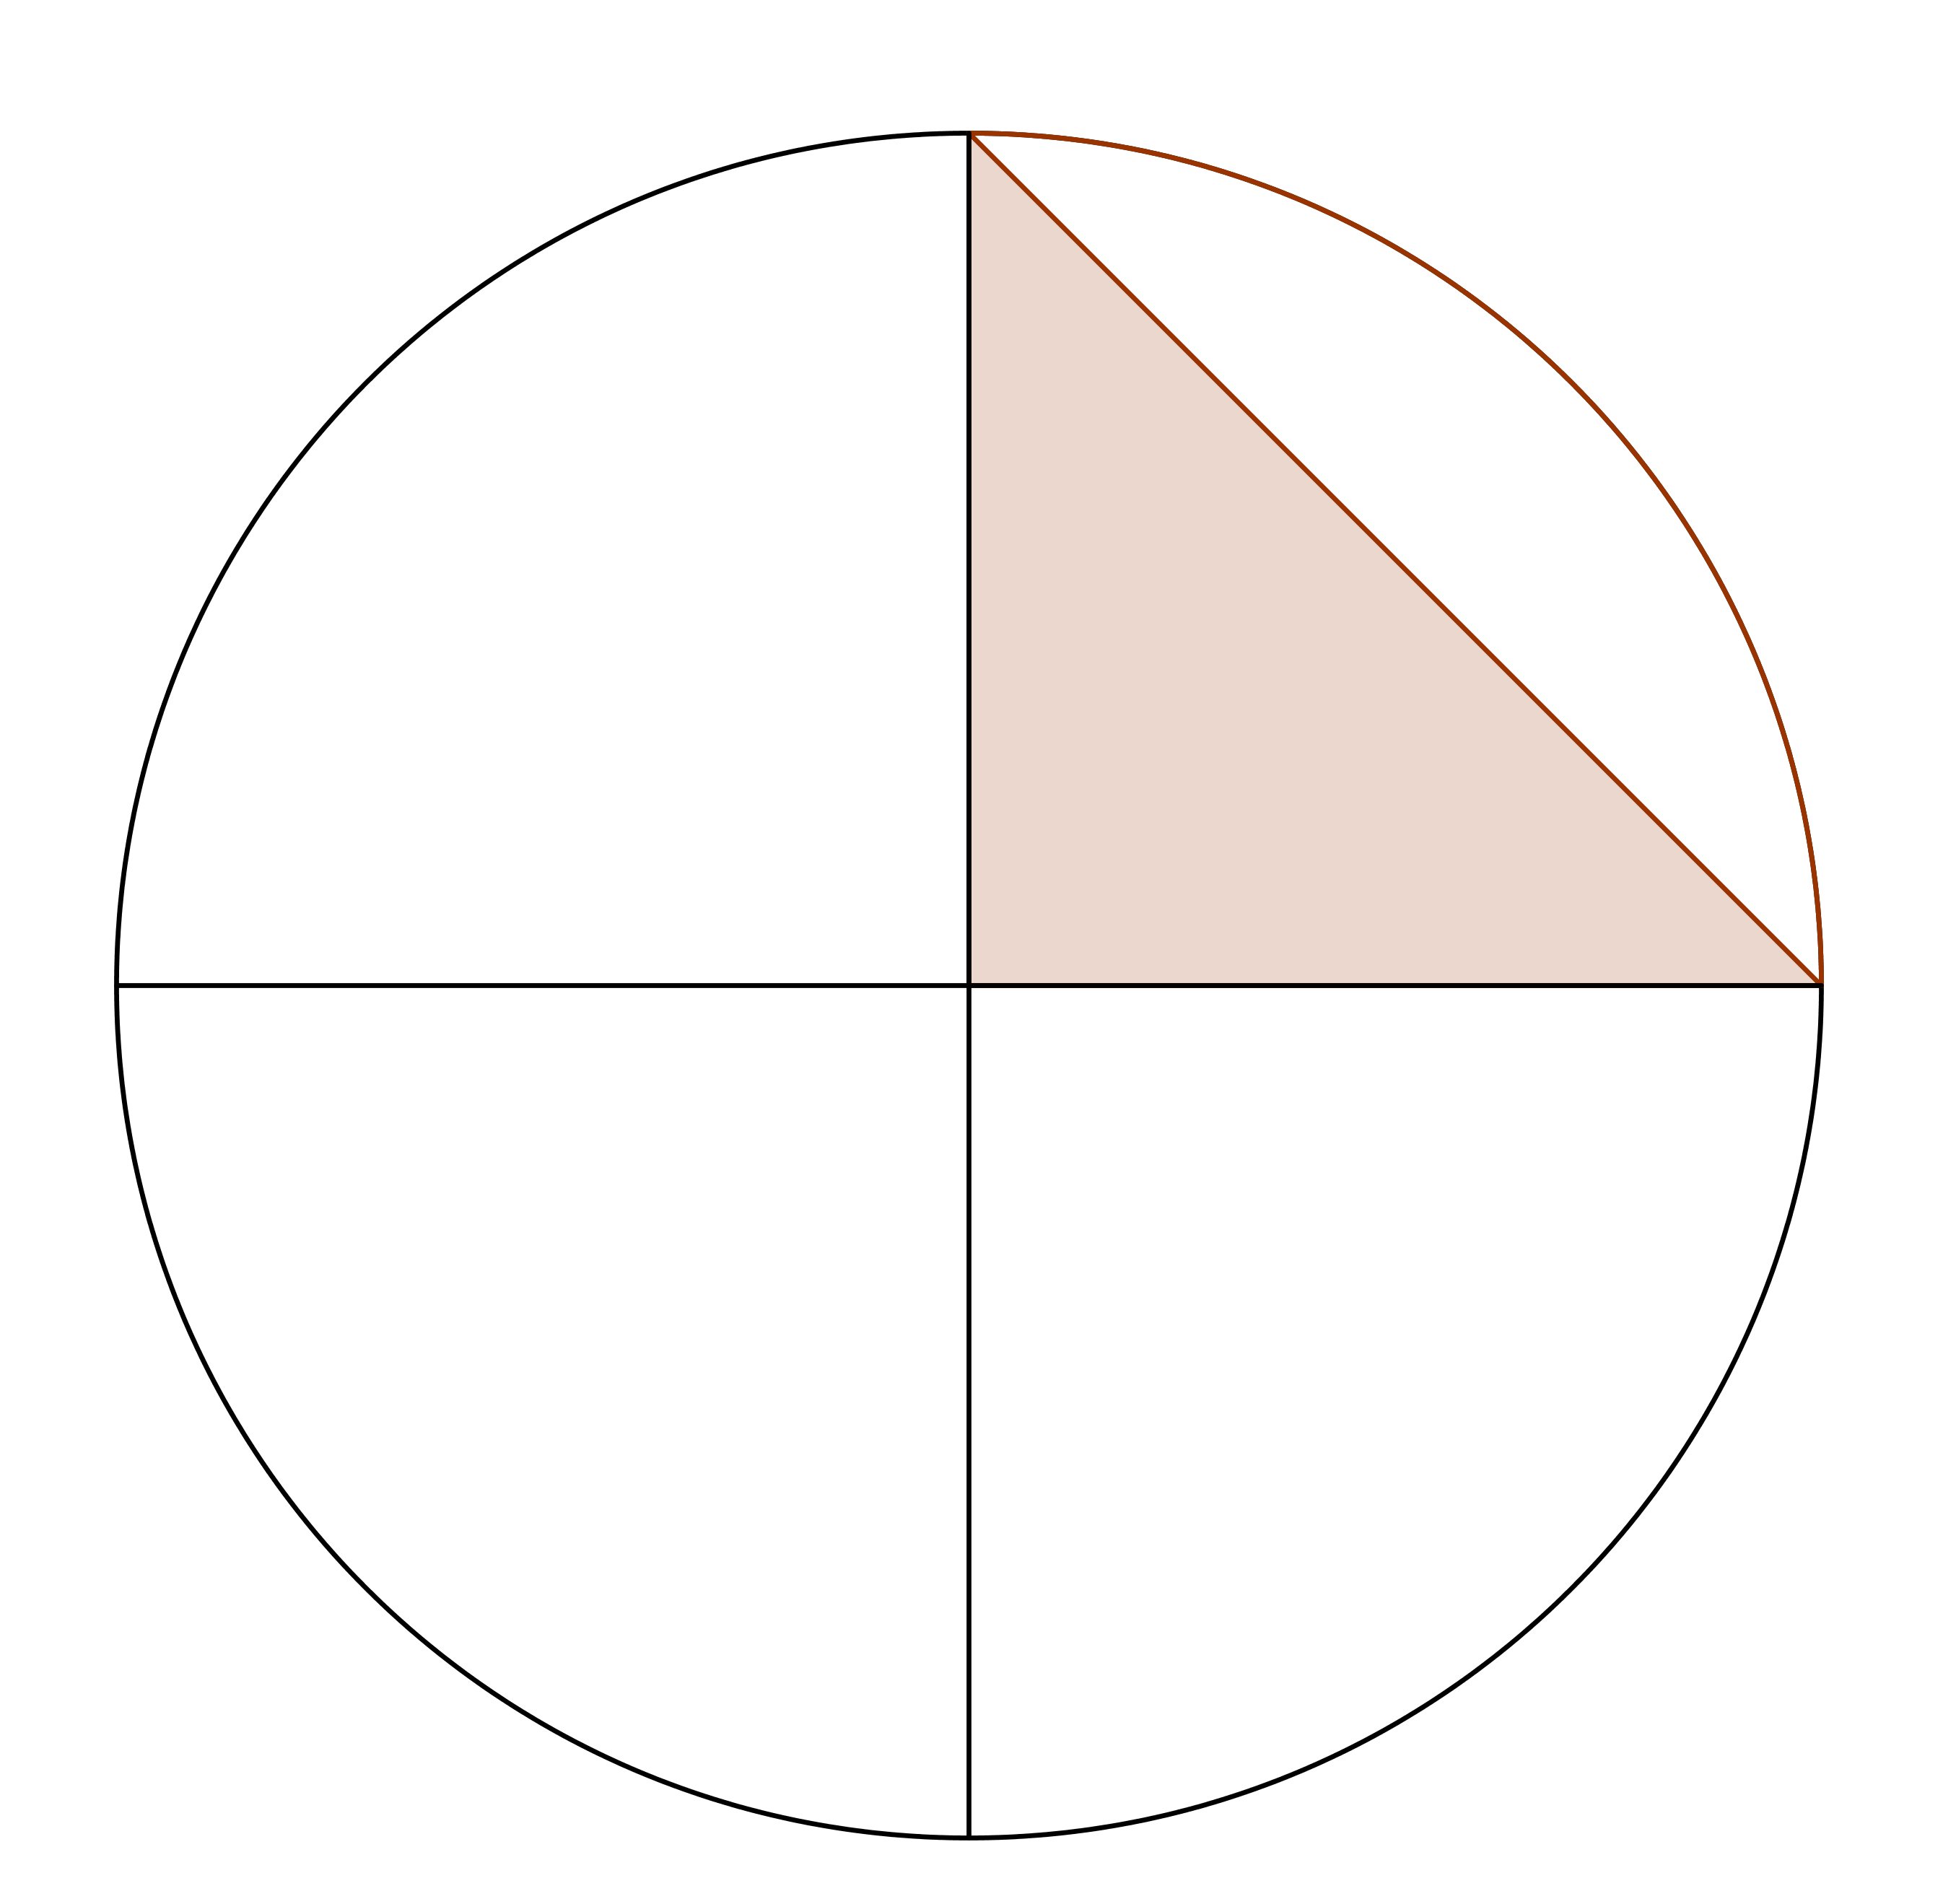
\includegraphics[width=0.3\textwidth]{08-4}
\end{figure}
\end{document}